%\addcontentsline{toc}{chapter}{Development Process}
\chapter{Design}

Design is the second step within the waterfall model \cite{waterfall}. This chapter will describe and provide reasons for the architectural design decision made throughout this project. This chapter will also include the steps that were taken to design the user interface.

\textit{\textbf{(Appendix. “Design Specification”)} For a more detailed description of the design for this project, please see the included appendix entitled “Design Specification”.} 

\section{Overall Architecture}
I intended to design the system in a modular format thus the system contains four main packages with each package containing a tests package. Keeping code modulated enhances the reusability of the code and also makes the code easier to maintain. In this section I will be listing each package and explaining their purpose within the application.


\begin{description}
	\item[Activities package] Activities are Android's views \cite{android}. An activity provides a method of displaying information on screen for the user. The activities package contains the implemented classes for the activities. 
	\item[Models package] The models package contains the model classes for each of the database tables. A model represents an item created from the database, for example a drug or a piece of information about a drug. Keeping all models within one package allows the models to be reused in other applications.
	\item[Data download package] The data download package contains the Robospice \cite{robospice} requests classes, which are responsible for downloading the individual API URLs and then parsing the data obtained. Each class within this package downloads a specific API XML file \cite{xml}. Having all the data download classes in one package makes it easy to add new classes to download additional data in the future.
	\item[Database package] The database package contains the class that is responsible for the interacting with the SQLite database \cite{sqlite}. This class is responsible for fetching, creating and deleting data from the database. Having this class within its own package will allow the database and database code to be reused within other applications. If the code within the database helper class becomes to large using a package will also allow the code to be broken into smaller classes.
	\item[Tests packages] Each package contains a package called tests. Within each test package is classes testing each class of the original package through both JUnit \cite{junit} tests and Android instrument tests.
	\item[XML edibility] As the application will be given to a team of developers who may not have extensive experience in Android development it was essential that I make the basics of the application editable by an inexperienced developer, to achieve this all string values have been set in one XML file (strings.xml) \cite{strings_xml}. Having done this, any text within the application can be changed by editing this XML file \cite{xml}. As this application is produced for NHS Wales \cite{nhs_website} they may in the future want to translate the application to Welsh, to adding Welsh language support would be relatively easy due to this design choice.

	To further improve the customisability of the application all API URL’s and the structure of the XML files is set within a single XML file (data\_download.xml) \cite{strings_xml}. This makes the task of changing API URL’s and the format of the data simple.

\end{description}

\section{Data storage}
One of the made decisions when designing the application was deciding how the data for the application would be stored, within this section I will discuss the possible methods of storing the data and why I chose the method I chose.

\subsection{Store the data as XML files}

Downloading the XML from the XML API URLs and storing the XML file \cite{xml} on the device was one of the methods I considered. This method would allow for a quicker download task, as the task would not have to parse the XML. This method would also ensure the data was exactly as it was downloaded.

This is not a great method of storing the data on the device, as the device would have to parse all the XML files every time the data was needed by the application. This method would also be slow at searching and ordering the data, as it provides no indexing functionality.

\subsection{Store the data as a serialised object}

For this method the application would parse the XML file \cite{xml} into Java \cite{java} objects and then save the object onto the device through serialisation. This method would be quicker at runtime than storing the as XML files as the data will already be parsed when opening the data. 

There are several issues with this method, the first issue being that this method does not allow indexing of the results and therefore searching the data will be slow. Another issue with this method is the entire dataset will need to be loaded into the devices memory whenever using the data, which could cause some devices to run out of memory.

\subsection{Store the data within an SQLite database}

The Android SDK \cite{android_sdk} comes with a set of libraries for creating and interacting with SQLite databases \cite{sqlite}. SQLite database can be indexed and are therefore quicker than the above-mentioned methods for searching the data \cite{sqlite}. 

I decided to use an SQLite database \cite{sqlite} to store the data for the application. The data is parsed from XML \cite{xml} into usable objects and then stored in the SQLite database. Using an SQLite database allow the application to only load needed data into memory when needed, by using the WHERE operator when searching for data. Using an SQLite database also helped keep the data in organised structure, which would allow the data to be used by other applications if needed. 

The main issue with using SQLite database \cite{sqlite} is that the stored data may be larger than if the data was stored as a serialised object, but if the size of the database became an issue the database could be compressed.

\subsection{Database design}
As it had been decided that a database would be used to store the data, the next step was to design the database structure. The database tables have been normalised into third normal form. SQLite foreign key constraints were only introduced into the Android SDK \cite{android_sdk} at API version 16, as I wanted the application to have the largest reach possible I decided not to use foreign key constraints and therefore monitor foreign key relations manually. 

The first table to be designed, was the drugs table. The purpose of this table is to contain all the drugs that are downloaded. Within the original designs I had planned to place all drug information within the drugs table, but as the drug information’s changed between drugs I decided it would be better to create a separate table for drug information’s.

\begin{center}
\begin{longtable}{|l|l|l|p{8cm}|}
\caption{Table showing drugs database table structure}\tabularnewline
\hline
\textbf{Table name} & \textbf{Data type} & \textbf{Allow null} & \textbf{Purpose}                                                                 \\ \hline
\uline{id}                  & Integer            & No                  & Holds the drugs ID that is set from the downloaded XML. This is the primary key. \\ \hline
name                & String             & No                  & Contains the drugs name.                                                         \\ \hline
\end{longtable}
\end{center}
The next table to be designed, was drug information’s table. The purpose of this table was to hold a single piece of information about a drug, such as the method of administration or the flushing guidelines. Some drug information’s also contain a header helper. Header helpers are extra help information explaining the header. These are displayed to the user upon clicking the header or information button next to the header.

\begin{center}
\begin{longtable}{|l|l|l|p{8cm}|}
\caption{Table showing drugInformations database table structure}\tabularnewline
\hline
\textbf{Table name} & \textbf{Data type} & \textbf{Allow null} & \textbf{Purpose}                                                                             \\ \hline
\uline{id}                  & Integer            & No                  & Holds the drug information id, this is an auto incrementing value. This is the primary key   \\ \hline
drug\_id*           & Integer            & No                  & The id of the drug this information belongs to. This is a foreign key to the drugs table id. \\ \hline
header\_text        & String             & No                  & The header for the piece of information                                                      \\ \hline
header\_helper      & String             & Yes                 & The helper information for the drug information if it exists                                 \\ \hline
section\_text       & String             & No                  & The main body of information for the drug information.                                       \\ \hline
\end{longtable}
\end{center}
The next table that was designed, was the drug indexes table. This table contains the drug indexes. A drug index is an extra name for a drug. A drug may have more than one index. The drug indexes are what the user will be shown in the list of searchable drugs.

\begin{center}
\begin{longtable}{|l|l|l|p{8cm}|}
\caption{Table showing drugIndexes database table structure}\tabularnewline
\hline
\textbf{Table name} & \textbf{Data type} & \textbf{Allow null} & \textbf{Purpose}                                                                             \\ \hline
\uline{id}                  & Integer            & No                  & Holds the drug information id, this is an auto incrementing value. This is the primary key   \\ \hline
drug\_id*           & Integer            & No                  & The id of the drug this information belongs to. This is a foreign key to the drugs table id. \\ \hline
name                & String             & No                  & The name for the index                                                                       \\ \hline
\end{longtable}
\end{center}

The final table to be designed, was the table containing the drug calculation information’s. This table contains all the information needed to perform the infusion rate or dosage calculations. As SQLite \cite{sqlite} does not support boolean types \cite{sqlite_dt} integer values (0 or 1) were used to represnt booleans. Integers representing booleans were used for if the patient weight required and if time is required columns.


\begin{center}
\begin{longtable}{|l|l|l|p{7cm}|}
\caption{Table showing drugCalculations database table structure}\tabularnewline
\hline
\textbf{Table name}   & \textbf{Data type} & \textbf{Allow null} & \textbf{Purpose} \\ \hline
\uline{id}                    & Integer            & No                  & Holds the calculators id, this is an auto incrementing value. This is the primary key        \\ \hline
drug\_id*             & Integer            & No                  & The id of the drug this information belongs to. This is a foreign key to the drugs table id. \\ \hline
infusion\_rate\_label & String             & No                  & The label used for the infusion rate calculator                                              \\ \hline
Infusion\_rate\_units & String             & No                  & The units of the calculated infusion rate.                                                   \\ \hline
dose\_units           & String             & No                  & The units of the calculated dose                                                             \\ \hline
patient\_weight\_req  & Integer            & No                  & If the patients weight is required for the calculation (1 represents true, 0 false)          \\ \hline
time\_req             & Integer            & No                  & If the time is required for the calculation (1 represents true, 0 false)                     \\ \hline
factor                & Integer            & No                  & The factor used within the calculation                                                       \\ \hline
\end{longtable}
\end{center}

\section{Downloading of data}

The next part of the design process was to decide how the data for the database would be downloaded. The download process had to be able to run in the background on the device as the download can take several minutes, therefore a user is likely to minimise the application. In this section I will discuss the methods of downloading the data that I considered.

\subsection{Download the data using an AsyncTask}

It would have been possible to download the data using an AsyncTask \cite{async_task} as they AsyncTasks create a new thread meaning they can be used for HTTP requests. Within the Android documentation it states that AsyncTasks should not be used for long running tasks (more than a few seconds) \cite{async_task}, due to this reason I decided not to use AsyncTasks for downloading the data. Another reason against using AsyncTasks is that they are attached to the activity that created them, so if the user minimises the application the task will also be killed, thus not allowing background downloading.

\subsection{Download the data using a service}

The Android documentation suggests using a service \cite{service} for any long running task \cite{async_task}. A service runs within its own thread therefore allowing the download to continue working whilst in the background.  A service will also place an item in the devices notification panel letting the user know that the service is still running. Using a service to download the data would have worked and been a good solution if implemented correctly.

A service is only a basic class for running a process in the background, it provides no implementation for alerting the view of its progress, nor does it contain any error handling should the tasks fail \cite{service}. The reason I chose not to download the data using a basic service is that I would need to implement a large amount additional code to handle all areas of failure and to notify the view of the downloads progress.


\subsection{Download the data using a Robospice service}

Robospice \cite{robospice} is an open source library released under the Apache licence \cite{apache_licence} that simplifies the implementation of long running tasks. Robospice runs on top of the Android service providing implementation for frequently used features needed when implementing services. Robospice makes notifying the view of progress simple and also allows for multi-threading meaning that simultaneous downloads can occur. Another useful feature that Robospice contains is its error handling features, it retries a task a set amount of times \cite{robospice} before finally alerting the main thread of its failure.

I decided that using a Robospice service to handle the downloading of data would be the best solution. Using a Robospice service meant I would be able to focus on the body of the task instead of worrying about implementing the various features needed for the service \cite{robospice}. Robospice does allow for caching, but as the data will only be downloaded once every few months I decided using an un-cached service would be acceptable.


\section{Design pattern used}

When planning the application it was planned to create the application using a Model-View-Controller (MVC) \cite{mvc} design pattern. Once I began developing within Android it became apparent that a true MVC approach was not possible within Android. Although a true MVC approach was not possible I attempt to follow the MVC pattern throughout my design, thus creating a package for models, a package for activities (views) and separate packages for everything else (controllers). I believe that by modulating the code, the maintainability and reusability of the code has been increased.

\section{Database interactions class}
A single database interaction class was designed. The purpose of this class was to handle all interactions with the database, thus keeping all SQL code into a single class. This class contains the method for creating and retrieving data, whilst also containing the methods for creating and updating the database.

I wanted to be able to test the all methods within the database class without altering the original database, to achieve this a separate constructor was creating which prepends a suffix to the database files name, thus making the test database separate from the original one.

Currently the amount of methods within this class isn’t very large, but if the application grows it would be a good idea to split this class into separate classes that handle different section of the database, for example a separate class for each table in the database.

\section{Download data singleton}
It had been decided that the downloading of data would be executed within a Robospice service \cite{robospice}. Robospice services like Android services run within there own thread \cite{robospice} and are therefore are not attached to a specific activity. Although Robospice services allow for the passing of progress from the service to the activity, they do not natively support the passing of data.

To pass data between the download services and the download activity I designed a singleton class. A singleton class is a class that can only have one object of itself instantiated \cite{singleton}. A method is created within the class for the purpose of retrieving the single instantiated object. Using a singleton for the download progress meant that both the service and the activity would be using the same object, thus allowing data to be passed between them.

\section{Calculation class}
The calculation class is the class responsible for handling the dosage and infusion rate calculations. I intended to create a powerful class that could handle both the validation and calculation of the calculations.

A method called validate was designed, this method checks that all data used for the calculation is present and correct. The method then returns an integer for the result of the validation. This integer can either represent an error (which the user must change), a warning (which the user has the option to change or continue) or success.

Once the validate method has been called, if the result is a success or a warning and the user opted to continue the calculation will be performed.

Keeping the validation and calculation within the same class means that the calculation code be reused within other projects. Using this approach also allowed for more rigorous testing as the validation and calculations could be tested together whilst Unit testing \cite{junit}.

\section{Preferences class}

Android provides developers with a class for storing values on the device \cite{android}. This class is called SharedPreferences. A shared preference \cite{shared_pref} is a key-value pair accessed by providing the key as a string. SharedPreferences are useful for storing single pieces of information on the device without creating a separate table in the database for them\cite{shared_pref}. Android also provides security on top of SharedPreferences, preventing other applications for accessing your applications SharedPreferences. 

The preferences class was used as a wrapper class for inserting, updating and deleting SharedPreferences. The preferences class is used within the application to store the users credentials, the date of the last database update and if the database was successfully downloaded.

Although Android provides some security for SharedPreferences \cite{shared_pref}, they cannot stop a malicious user from accessing the data should they have physical control of the device. Therefore it is important that secure information is not stored within the preferences without being encrypted.

\section{Authentication class}

This class was designed to provide authentication with the NHS server. This class contains methods for validating a users username and password and retrieving the user credentials so that they can be used when updating the database. The authentication class also provides a method for checking whether a user is logged in, this is used when the application is first opened and decides if the login or main view should be opened.

\section{Splash activity}
When the application first opens the application has to decide whether to open the login screen, the main screen or the update screen. Android does not allow any logic to be processed before the first activity is displayed. This caused an issue, as there was no way of opening the correct activity without first opening an activity.

One solution to this problem would be put the logic within the main activity and if the user needed to login or download the database they could be redirected. This would not be an ideal solution as for a brief amount of time the main activity would be opened, causing a flicker.

I decided that designing a splash activity would be the best way to solve this problem. The splash activity briefly displays the NHS \cite{nhs_website} logo on a neatly presented background whilst the application decides where to redirect the user, the user is then redirected to the correct screen, without any flickering.

\section{Common activities}
Android provides the user with menu options when the user presses the menu button on the device \cite{android}. This menu contains items such as update, logout and exit. The menu buttons in most applications vary between activities, but within this project the menu items are the same throughout the application, the only time they change is when the user is logged out. 
It is possible to create the menu item’s manually within each activity but I wanted to design the application so that the code is DRY. To achieve this I created a class that inherited Androids Activity class and implemented the Exit and About buttons for that class, this class could then be inherited within activities that needed to display the Home and About buttons. I then created an another class which inherited from that class adding buttons that can be shown once the user is logged in (Logout, Home, Browse, Calculator, Update). 

Using this approach makes it easy to add items to the menu of all activities. If an activity needs a custom option adding to the menu this can be done easily within the activity.

\section{User interface design}

I planned to design an application that was both aesthetically pleasing and easy for the novice user to use. Within this section I will discuss how the user interface design decision were made and then display the user interface mock-ups that were created.

\subsection{Logo design}

An easily recognisable icon allows a user to find an application quickly without have to read the name of the application. Android uses the applications logo icon throughout the application \cite{android}. I wanted to create a logo that looked similar to other applications whilst still being unique enough to stand out. I searched the FindIcons website \cite{findicons} to find an icon that represents medication that was released under a commercially free licence. I then opened the icon in Photoshop, applied a circular background and added effects to the background and icon. The icon was then saved as a variety of sizes to be used on screens of varying densities.

\subsection{Android developer design guidelines}

During the background and analysis stage of the project I read the majority of the design guidelines \cite{android_design} laid out by Android. These guidelines taught me how to create applications that would scale for a multitude of devices whilst only implementing the design once. 

The guidelines \cite{android_design} taught me to use density-independent pixels (dp), for expressing layout and positioning of view object that need to scale as the density increases. If you were to layout an object using normal pixels, the object would use the same amount of pixel no matter how large the screen was, thus if viewing on a large screen with a large amount of pixels the object would appear small. Using density-independent pixels means the object will automatically scale as the density of the screen does.

I also learnt to use scale-independent pixels for fonts and text \cite{android_design}. Scale-independent pixels act just like density-independent pixels but they also scale for the users font setting, thus allowing the font to be larger if the user sets a large font within their device settings. Using scale-independent pixels increasing the accessibility of the application.
The guidelines also taught me about layout parameters such as match parent and wrap content. Match parent makes the layout parameter an object match its parents width or height \cite{android_design}. Using match parent is useful when you want a button to fill then the screen. The wrap content layout parameter allows the size of the views width or height to expand depending on the size of its contents This is useful when displaying information to the user which may be more than one line. 

Using these learnt Android design techniques allowed me to design a user interface that is fluid and expands well over a multitude of device size, of varying densities. They also allow the views to be rotated depending on the devices orientation automatically.

\subsection{Designing the interface to be easy to use}

In order to ensure that the user interface was easy to use, it was decided that the standard Android user interface library would be used. Using the standard user interface library \cite{android_design} ensured that a user familiar with the Android operating system would instinctively be able to use the application. To further improve the ease of use of the application I designed a main screen, which opens when the user first launches the application. The main screen describes the main functionality of the application and provides buttons that link to these functions.

\subsection{Making the application aesthetically pleasing}

To make the application as aesthetically pleasing as possible I adapted a simplistic design using a similar colour scheme to other NHS branded services. Simplistic designs have been becoming increasingly popular on the web, as they allow the user to focus on content rather than be distracted by fancy graphics. As the information contained within the application is the most important aspect of the application I decide that a simplistic design would be the best-suited design.

After creating the simplistic design I wanted to keep the user interacted by preventing the application content from being dull. To achieve this I changed the colour scheme of the applications action bar to match the standard NHS \cite{nhs_website} blue. This brightened up the application without distracting the user from the main content.

 
\subsection{Searching for drugs}
When the user navigates to the browse drugs page they are presented with a list containing the complete list of drug indexes. The user can scroll through this list to select a drug that they would like to view. As the list contains over 3000 drugs finding a specific drug manually would take a long amount of time. To solve this issue I designed a search box that would be displayed above the list of drugs, when the user enters text into the search box the list of drugs is filtered to only display drugs that match the searched text. This greatly improves the speed at which a user finds a wanted drug.

\subsection{Designing the view drugs page}
The main challenge when designing the user interface was how to best display the drug monographs \cite{monograph} to the user. The information contained within drug monographs can be quite large and therefore challenging to fit onto a mobile device’s screen. Another challenge added to the designing of the interface was the header helpers. Header helpers are extra information on a header explaining its contents. The view drug page had to have a method of showing that a header has help information and must allow the user to access this information. There were several different methods considered for displaying the information, within this section I will describe each solution that was considered and conclude with the chosen design.

The initial idea and the one provided by the NHS within their mock-ups was to have a view drug page that contained only the drug name and clickable headers, were the clickable headers lead the user to a new page containing the information within that header. This approach would’ve allowed the data to be displayed to the user and would’ve fit nicely on a mobile screen. Although this approach would’ve been suitable for displaying the information, I believe it would not have been a practical solution, as if the user needed information from multiple headers they’d have to navigate into each header individually.

The next design that was considered was similar to the above design, but instead of opening the information within a new page, the information would expand down from the header once the user clicked the header. This design would allow the user to view all the information that they needed at once and it would fit appropriately on a mobile screen.  One issue with this approach was that I could not think of a method for showing that the header contains helping information.  

The final chosen design was to display the entire drug information in one scrollable screen, using left indents to separate headers and content. This would allow the user to view all the needed within one screen. This design also meant that I could use an information icon next to headers with helper information to show that extra information is available. The on click event of the icon or header text can then be used to also open the helper information.

When the user clicks to view the helper information, an alert dialog box is shown containing the information. Alert dialogs open on top of the current screen and contain a close button to close the dialog \cite{android_design}. Using a dialog allows the information to be displayed to the user, without them navigating away from the view drug page.

\subsection{Designing the calculator page}
The calculator page is the screen that is used to calculate dose and infusion rates. It is extremely important that the calculated values are correct and therefore the calculator page must be easy for the user to use thus decreasing user errors. 

I wanted to keep the calculator page simple, hence why the calculator and view drug page were separate pages. To ensure that the user knew which drug they were currently calculating for, I designed the page so that the drug name was shown in the action bar and within a bold header above the calculator.

The next step in designing the user interface to be easy to use, was to ensure that only inputs that are needed for the calculation are shown. When the user changes between dose and infusion rate calculations, the inputs that are no longer needed are hidden.

To ensure that the user entered the correct values, above each input field is a label describing the input and the units (E.g. Patient weight, kg). This reassures the users that they’re using the correct field and that they’re using the correct units. Each input also restricts the users keyboard to a decimal keyboard, ensuring the user can only enter numerical values.

To further improve the reliability of the calculator page warnings and errors are shown to the user. Errors are shown when the data enter is not valid, for example a patients weight being less than 0. Warnings are displayed to the user when the value entered seems incorrect, giving the user the option to change the value or to continue with the inputted value.

\subsection{Showing the calculation}
Once the user has entered the values for the calculation and clicked the calculate button they will be displayed with the calculated answer. I decided to use an alert dialog \cite{dialog} to display the calculated answer. This allows the user to view the answer without leaving the calculator page. 

To ensure that the calculation has been calculated correctly I decided to show the original equation used to calculate the dosage, then show the equation with the users entered values and then finally display the answer. This allows the NHS staff member to ensure the application is using the correct equation and also allows them to perform the calculation manually themselves. I believe this approach will improve the NHS's confidence within the application.

\section{User interface mock-ups}
After deciding the features of the design I began creating user interface mock-ups. User interface mock-ups allow you to quickly test a variety of designs without having to complete a detailed design. Mock-ups were created for the application to test designs for each view within the application. Within this section I will list all the user interface mock-ups that were created. The mock-ups within this section were created using LucidCharts \cite{lucid_charts}.

\begin{figure}
\centering
\begin{minipage}{.5\textwidth}
  \centering
  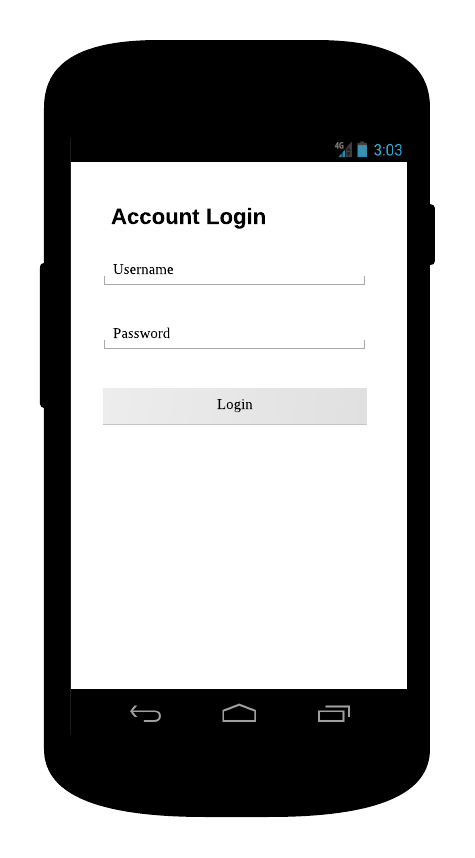
\includegraphics[width=.7\linewidth]{Images/mockups/login.png}
  \captionof{figure}{Login activity mockup}
\end{minipage}%
\begin{minipage}{.5\textwidth}
  \centering
  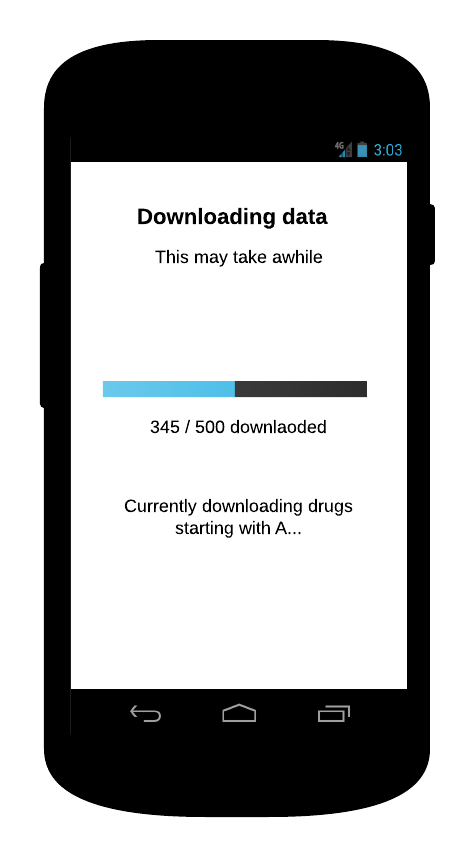
\includegraphics[width=.7\linewidth]{Images/mockups/download.png}
  \captionof{figure}{Download activity mockup}
\end{minipage}
\end{figure}

\begin{figure}
\centering
\begin{minipage}{.5\textwidth}
  \centering
  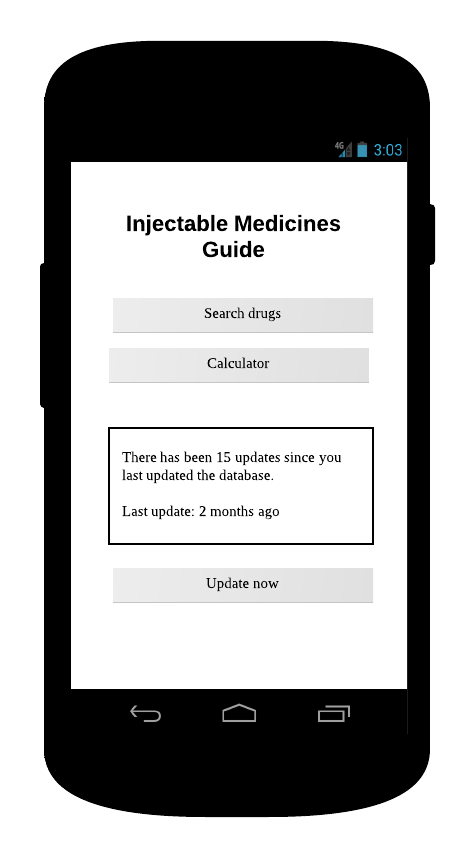
\includegraphics[width=.7\linewidth]{Images/mockups/main.png}
  \captionof{figure}{Main activity mockup}
\end{minipage}%
\begin{minipage}{.5\textwidth}
  \centering
  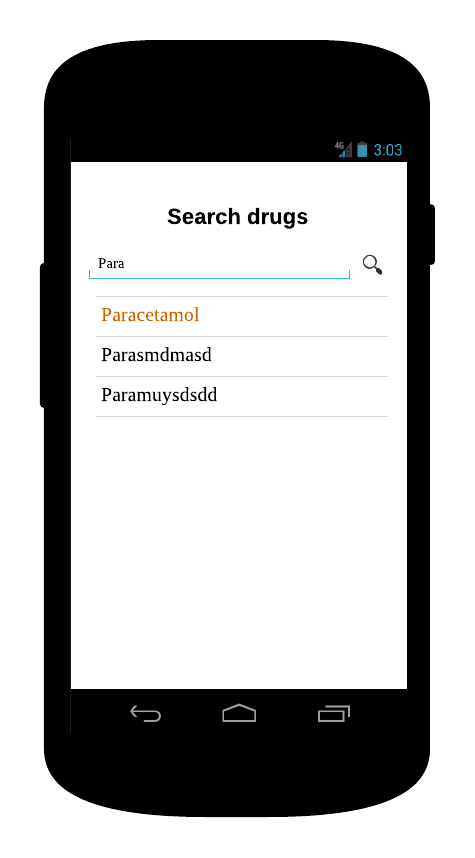
\includegraphics[width=.7\linewidth]{Images/mockups/browse.png}
  \captionof{figure}{Browse drugs activity mockup}
\end{minipage}
\end{figure}

\begin{figure}
\centering
\begin{minipage}{.5\textwidth}
  \centering
  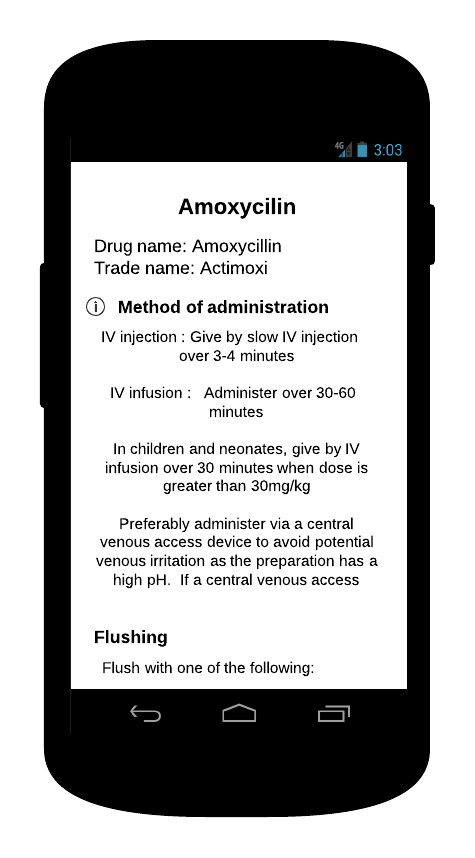
\includegraphics[width=.7\linewidth]{Images/mockups/viewDrug.png}
  \captionof{figure}{View drug activity mockup}
\end{minipage}%
\begin{minipage}{.5\textwidth}
  \centering
  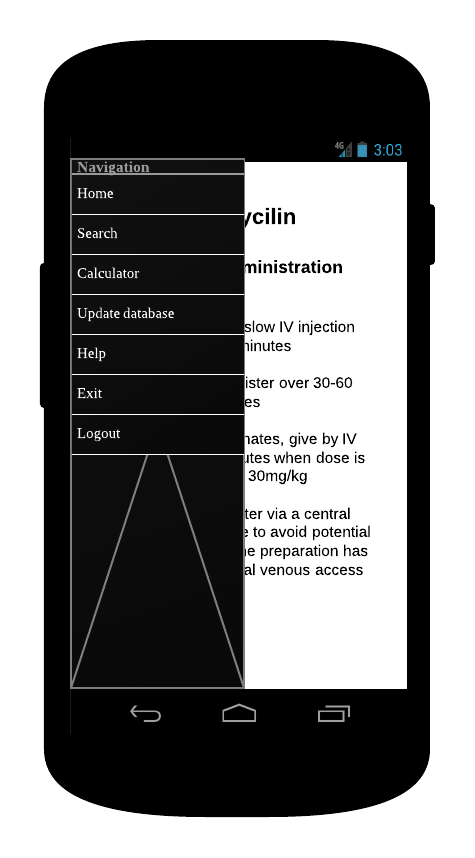
\includegraphics[width=.7\linewidth]{Images/mockups/menu.png}
  \captionof{figure}{Menu mockup}
\end{minipage}
\end{figure}

\begin{figure}
\centering
\begin{minipage}{.5\textwidth}
  \centering
  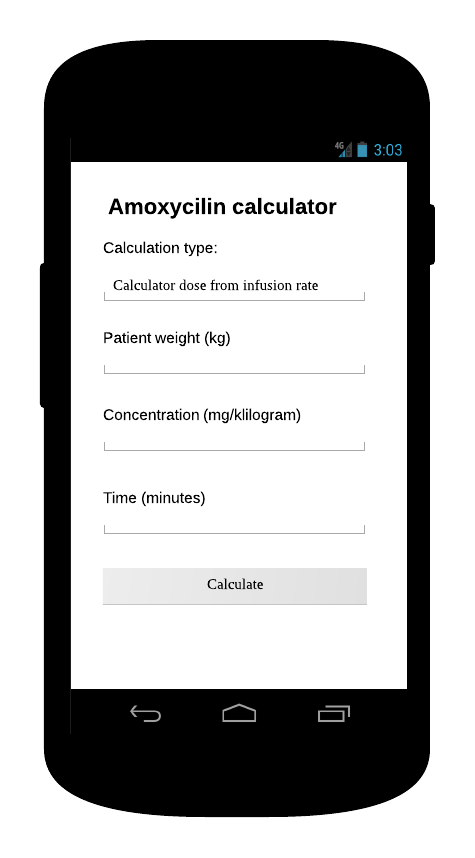
\includegraphics[width=.7\linewidth]{Images/mockups/calc.png}
  \captionof{figure}{Calculator activity mockup}
\end{minipage}%
\begin{minipage}{.5\textwidth}
  \centering
  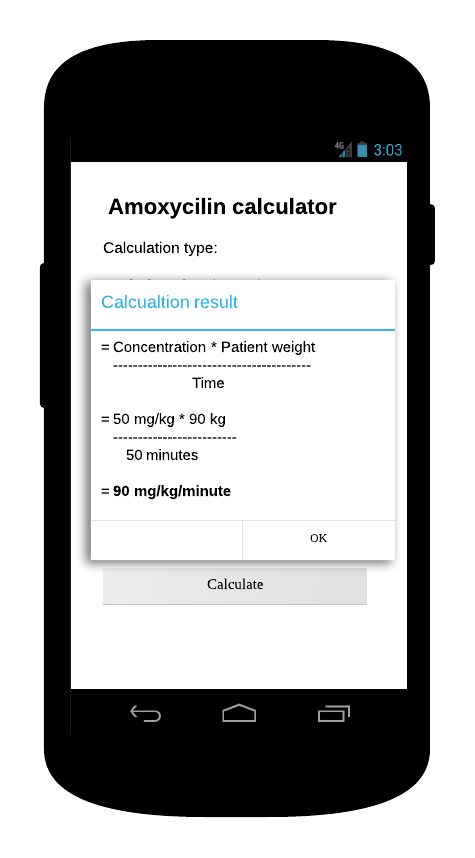
\includegraphics[width=.7\linewidth]{Images/mockups/calcDisplay.png}
  \captionof{figure}{Calculator display mockup}
\end{minipage}
\end{figure}



\begin{description}
	\item[Login screen]
	This is the first screen the user sees when opening the application for the first time. Once they login their details are saved so they should only have to login once.
	\item[Download screen]
	This page is shown when the user is downloading the database for the first time, or when they are updating the database. The tasks within this screen can take several minutes so a progress bar helps to show to the user that the task is still running and hasn’t crashed.
	\item[Main screen]
	Shown once the user has successfully downloaded the database. This is the first screen a reoccurring user is sent to. This page allows the user to navigate to other screens.
	\item[Browse drugs / calculators screen]
	These two screens are very similar; they both display a list of drugs and allow you to filter the list by entering part of the drugs name, inside the search box. The browse drugs page contains a list of all drugs and the browser calculators screen shows all drugs that have calculators.
	\item[View drug screen]
	This screen is displayed when the user selects a drug from the browse drugs page. It contains the complete monograph for the drug, some headers contain an icon next to the header, if the user clicks a head with this icon, and helper information for that header is displayed within a dialog.
	\item[Calculator screen]
	This is the screen where the user enters patient information and is displayed with the either the dose or infusion rate for the drug. When the result of the calculation is displayed, the equation used to perform the calculation is also displayed and described.
	\item[Options menu]
	The options menu is displayed when the user presses the menu button on their device. This menu is designed to allow the user to quickly navigate to useful parts of the system from any screen of the system.
\end{description}


